%!TEX root = kotov.tex
\section{Task 3}
\begin{task}
    Про фирму
\end{task}

\begin{solution}
    \begin{remark}
        Не успею сделать поясняющих рисунков :ссс
    \end{remark}

    Рассмотрим возможные стратегии принятия решений. Пусть мы сейчас работаем над заказом $i$ и нам приходит новый заказ $i+1$. Тогда нам надо решить, что эффективнее: довершить текущий заказ или бросить его и начать делать новый? Посмотрим эти два варианта с точки зрения суммарного времени окончания этих двух заказов:
    \begin{gather}
        \label{eq:times}
        \underbrace{r_i + t_i}_{\text{окончание 1-ого}} + \underbrace{r_i + t_i + t_{i+1}}_{\text{окончание 2-ого}} \lessgtr \underbrace{r_{i+1} + t_{i+1}}_{\text{окончание 2-ого}} + \underbrace{r_{i+1} + t_{i+1} + t_{i} - r_{i+1} + r_i}_{\text{окончание 1-ого после 2-ого}} \\
        r_i + t_i \lessgtr r_{i+1} + t_{i+1}
    \end{gather}
    Если $r_i + t_i < r_{i+1} + t_{i+1}$, тогда выгоднее закончить текущий заказ, иначе, выгоднее начать делать новый. То есть мы можем ввести приоритет заказа $p_i = r_i + t_i$ и сравнивать по нему.

    Но что с другими заказами? Тут просто, всего у нас возможно условно три состояния:
    \begin{enumerate}[1)]
        \item Штатно закончили просто $i$-ый заказ, тогда из массива заказов в ожидании берем минимальный по приоритету, если таковые заказы есть
        \item Пришел новый заказ:
        \begin{enumerate}[a)]
            \item Если выгоднее продолжать делать текущий заказ, то помещаем новый заказ в массив ожидания.
            \item Если выгоднее начать делать новый заказ, то помещаем текущий заказ со своим приоритетом в массив ожиданий и начинаем делать новый заказ.
        \end{enumerate}
    \end{enumerate}
    Наивно можно просто каждый раз за $\O(n)$ брать минимум из массива, тогда это будет $\O(n^2)$, но можно завести кучу для приоритетов, тогда добавлять новые заказы будем за $\O(\log n)$ и вытаскивать минимум тоже за $\O(\log n)$, что приведет к $\O(n\log n)$.
\end{solution}
\begin{upd}
    Не совсем понял замечания, но поясню на словах чуть более подробно.
    Фирма может находится в двух состояниях: либо делает заказ, либо отдыхает. Второй случай не интересный, поэтому оставляем только первое состояние. Для этого состояния у нас могут быть различные ситуации, но для какой-то ситуации в вакууме предположим, что фирма работает над самым приоритетным (с точки зрения суммы окончания времени работы, конкретный вид приоритета обсудим позже) заказом под номером $i$.
    
    Предположим, что никаких новых заказов в процессе не поступило, тогда мы просто переключаемся в ``замороженный'' заказ, следующий по приоритету (такие заказы мы храним в каком-нибудь массиве).

    Если же в процессе выполнения заказа, приходит новый заказ, то мы должны решить, приоритетнее ли сделать его сейчас или лучше отложить, для этого я привел \eqref{eq:times}, в котором сравниваются в общем виде времена окончания текущего (самого приоритетного на данный момент заказа) с новым в этих двух ситуациях. Поясню это неравенство:
    \begin{figure}[H]
        \centering
        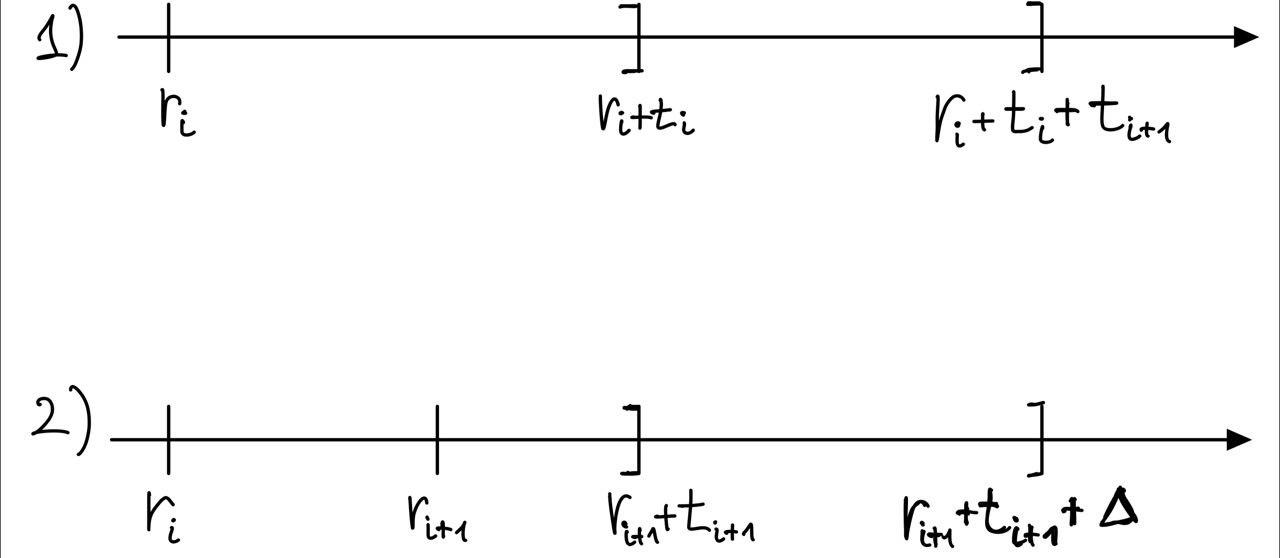
\includegraphics[width=\textwidth]{pics/photo_2020-10-10_13-15-11.jpg}
        \caption{Различные ситуации времени окончания заказов: вертикальная черта --- время начала заказа, закрывающая квадратная скобка --- время окончания заказа. $1)$ сначала доделываем текущий, потом следующий (формально взятый по приоритету из массива ожидающих заказов), $2)$ переключаемся на новый, а потом берем старый заказ. Считаем, что мы сразу переключаемся на выполнение очередного заказа, после выполнения текущего заказа.}
    \end{figure}
    \begin{remark}
        Вообще говоря, так как $i$-ый заказ был приоритетнее, чем все остальные, то при его замене на новый заказ, $i$-ый все также будет самым приоритетным заказом среди всех ожидающих выполнения заказов, поэтому в этой ситуации мы можем после выполнения новоприбывшего заказа просто переключиться на старый $i$-ый заказ.
    \end{remark}
    Теперь в \eqref{eq:times} посокращаем подобные слагаемые и получим очень простое неравенство $r_i + t_i < r_{i+1} + t_{i+1}$, результат которого будет говорить нам, стоит ли бросать текущий заказ ради нового. То есть приоритетом, как бы странно это ни звучало, но так следует из \eqref{eq:times}, можно считать $p_i = r_i + t_i$, и считать заказы, у которых $p_i$ меньше, приоритетнее.
    \begin{remark}
        Можно было бы подумать, что надо обновлять приоритеты у старых заказов, когда мы резко переключаемся на новый, но на самом деле это не нужно, так как это до сих пор сдвиг на одну и ту же константу всего массива, что не меняет их положение между собой.
    \end{remark}
    \begin{remark}
        Этот подход пока никак не учитывал способ хранения ожидающих заказов: для получения наиболее оптимального (в плане условий задачи подпункт b) можно использовать min-кучу.
    \end{remark}
    \begin{remark}
        Так как тут рассмотрена какое-то состояние в процессе работы фирмы, то приход нового заказа, когда мы делаем новый заказ, это все равно ситуация, в которой мы делаем какой-то текущий заказ и приходит новый заказ, при этом у нас есть какое-то количество заказов в ожидании.
    \end{remark}
\end{upd}
\begin{upd}
    Так, кажется, что это решение несколько контринтуитивно, вероятно, есть какой-то нюанс, который я не вижу, но, вроде бы, придумал другое решение: давайте хранить тогда в массиве оставшееся время выполнения заказа, в целом это не влияет на тот способ принятия решения о продолжении работы над текущим заказом или о переключении на новый (можно мыслить это так, что как будто нам в очередной момент приходит не один заказ, а сразу два: новый и текущий, но оставшимся $t$), тогда принимать решение будем совсем просто --- будем брать минимум такого массива, ну и наивный проход взять минимум из массива за линию в итоге даст в худшем случае $\O(n^2)$, а если хранить заказы в min-куче, то в худшем случае будет $\O(n\log n)$.
    \begin{remark}
        Но если мы и так работали над самым оптимальным заказом, то надо лишь определить будет ли новый заказ оптимальнее, чем текущий, так как на момент начала работы над текущим самым оптимальным заказом его оставшееся время выполнения и так было минимальным среди всех ожидающих заказов.
    \end{remark}
\end{upd}